\chapter{GroundOne: metodo e implementazione}
\label{sec:method}

% Source notes: Project/docs/thesis_notes.md (Ch. 3), Project/docs/dataset_plan.md §8, implementation_plan.md §4.

GroundOne è un modello linguistico compatto usato come System One. Legge una sola volta il documento e la risposta e,
senza generare testo, emette un verdetto per ciascuna frase valutata della risposta, ricavandolo dai logit di poche
lettere di risposta. Il capitolo descrive anzitutto la decisione che il modello prende e il prompt che raccoglie in un
unico forward pass tutte le decisioni relative a una risposta. Presenta poi l'obiettivo di addestramento, la
calibrazione delle probabilità in uscita e la regola che converte le probabilità nelle etichette restituite, e si chiude
con il software che implementa il tutto.

\section{Task e decisione}
\label{sec:method-task}

Per ogni frase di una risposta, GroundOne sceglie fra tre classi, definite nella Sezione~\ref{sec:data-task}: rispetto
al documento, la frase è \emph{supportata}, \emph{contraddetta} o \emph{non menzionata}. Alle tre classi corrispondono
le lettere A, B e C, e il modello restituisce una probabilità per ciascuna. Il punteggio binario di groundedness e le due
policy di segnalazione, strict (che segnala ogni frase non supportata) e lenient (che segnala soltanto le contraddette),
non sono domande distinte poste al modello. Vengono calcolati a partire da queste tre probabilità, e quindi un unico
forward pass basta per ogni utilizzo. Interrogare il modello direttamente sulle policy non porterebbe nulla, perché
ciascuna è una funzione deterministica della classe a tre vie. Domande separate moltiplicherebbero le decisioni senza
aggiungere informazione, e potrebbero inoltre fornire al modello obiettivi di addestramento incoerenti per la stessa
frase.

\section{Tutti i verdetti in un solo forward pass}
\label{sec:method-readout}

Il prompt contiene una breve istruzione, il documento e la risposta. Le frasi della risposta sono numerate, e ogni frase
a cui è associata una decisione è seguita da un marker, cioè da una breve stringa fissa che indica il punto in cui
leggere il verdetto: la stringa ``\texttt{~Verdict:}''. Le frasi prive di contenuto verificabile
(Sezione~\ref{sec:data-construction}) restano nel testo come contesto, ma senza marker. Il modello elabora l'intera
sequenza una sola volta. In corrispondenza dell'ultimo token di ciascun marker si leggono i logit delle lettere A, B e C,
che vengono normalizzati con una softmax\footnote{La \emph{softmax} trasforma un vettore di punteggi in una
distribuzione di probabilità: ogni punteggio $z_i$ diventa $e^{z_i} / \sum_j e^{z_j}$. Restringerla a tre lettere
significa calcolarla soltanto sui loro tre logit, ignorando il resto del vocabolario.} ristretta a queste tre lettere.
In un decoder ogni posizione vede soltanto quelle precedenti, quindi il verdetto sulla frase $i$ dipende dal documento e
dalle frasi $1, \dots, i$. È esattamente ciò che serve alla verifica, perché i riferimenti, come i pronomi, puntano
all'indietro. Quanto segue l'ultimo marker non influisce su alcun verdetto, quindi la sequenza si chiude lì. La Figura~\ref{fig:method-marked} mostra la struttura del prompt e i punti in cui avviene il readout.

\begin{figure}[htbp]
\centering
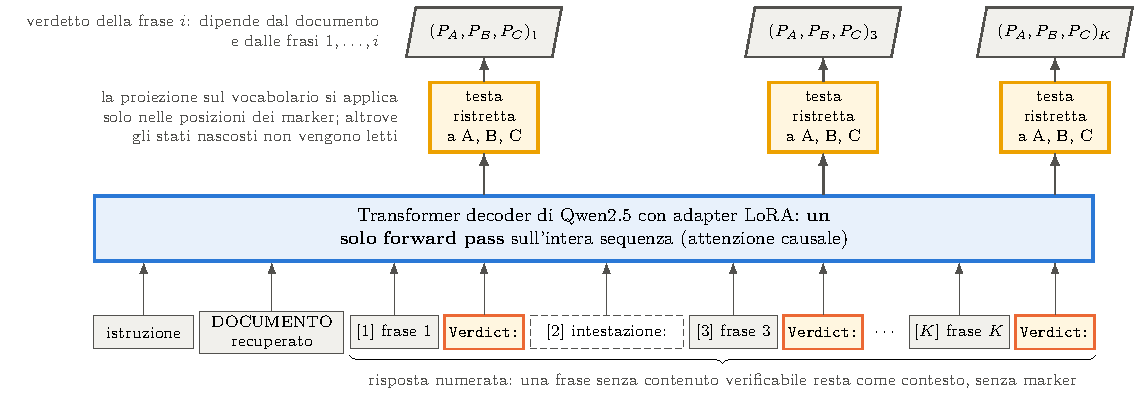
\includegraphics[width=\textwidth]{images/diagrams/method_marked_prompt_tikz.pdf}
\caption{Il prompt a marker di GroundOne (design b). Le frasi della risposta sono numerate e ogni frase valutata è seguita dal marker ``\texttt{~Verdict:}''; una frase senza contenuto verificabile (qui un'intestazione) resta come contesto, senza marker. Il modello elabora l'intera sequenza in un solo forward pass, e la testa di output, ristretta alle lettere A, B e C, si applica soltanto nelle posizioni dei marker. Per l'attenzione causale il verdetto della frase $i$ dipende dal documento e dalle frasi da 1 a $i$.}
\label{fig:method-marked}
\end{figure}

Due accorgimenti rendono il readout esatto ed efficiente. Il primo riguarda l'esattezza: il prompt viene costruito
tokenizzando separatamente le sue parti e poi concatenandole, così che la posizione di ogni marker sia nota con
esattezza e resti identica in addestramento e in inferenza. Il secondo riguarda l'efficienza: la proiezione di output
sul vocabolario si applica solo nelle posizioni dei marker. Il corpo del transformer elabora l'intera sequenza, ma la
grande matrice del vocabolario viene moltiplicata soltanto per i pochi stati nascosti effettivamente letti, cioè per i
vettori che il modello calcola nelle posizioni dei marker.

La lettura a marker determina anche il costo di una verifica. Si indichino con $S$ la lunghezza complessiva di documento
e risposta, con $K$ il numero di decisioni e con $m$ la lunghezza in token di un marker. Il System One richiede un solo
prefill di $S + K m$ token. Un giudice generativo, invece, deve anche produrre i propri verdetti in fase di decoding. Se
ogni verdetto richiede $n$ token e ogni token in decoding richiede un tempo $t_\mathrm{dec}$, il costo del giudice è
all'incirca $\mathrm{prefill}(S) + K\, n\, t_\mathrm{dec}$. La lunghezza $m$ di un marker è di soli tre token, mentre sull'hardware di
riferimento il decoding è molto più lento del prefill a parità di token; il divario fra i due costi, quindi, si allarga
al crescere di $K$. Sull'M4 usato in questa tesi, con il modello 0.5B il prefill costa circa 0.37\,ms per token e il
decoding 5.9\,ms per token generato; con il 3B i due valori sono 2.2 e 31.8\,ms. Un token in decoding costa quindi
quanto quattordici-sedici token in prefill. Le due fasi, inoltre, sollecitano l'hardware in modo diverso. Il prefill
elabora molti token insieme ed è limitato dalla capacità di calcolo, mentre il decoding produce un token alla volta ed è
limitato dalla banda necessaria a leggere i pesi~\cite{pope2023scaling,patel2024splitwise}. La differenza riemerge nelle
misure di energia del Capitolo~\ref{sec:results}. La Figura~\ref{fig:method-cost} traduce il modello di costo in secondi per risposta, usando soltanto queste costanti misurate.

\begin{figure}[htbp]
\centering
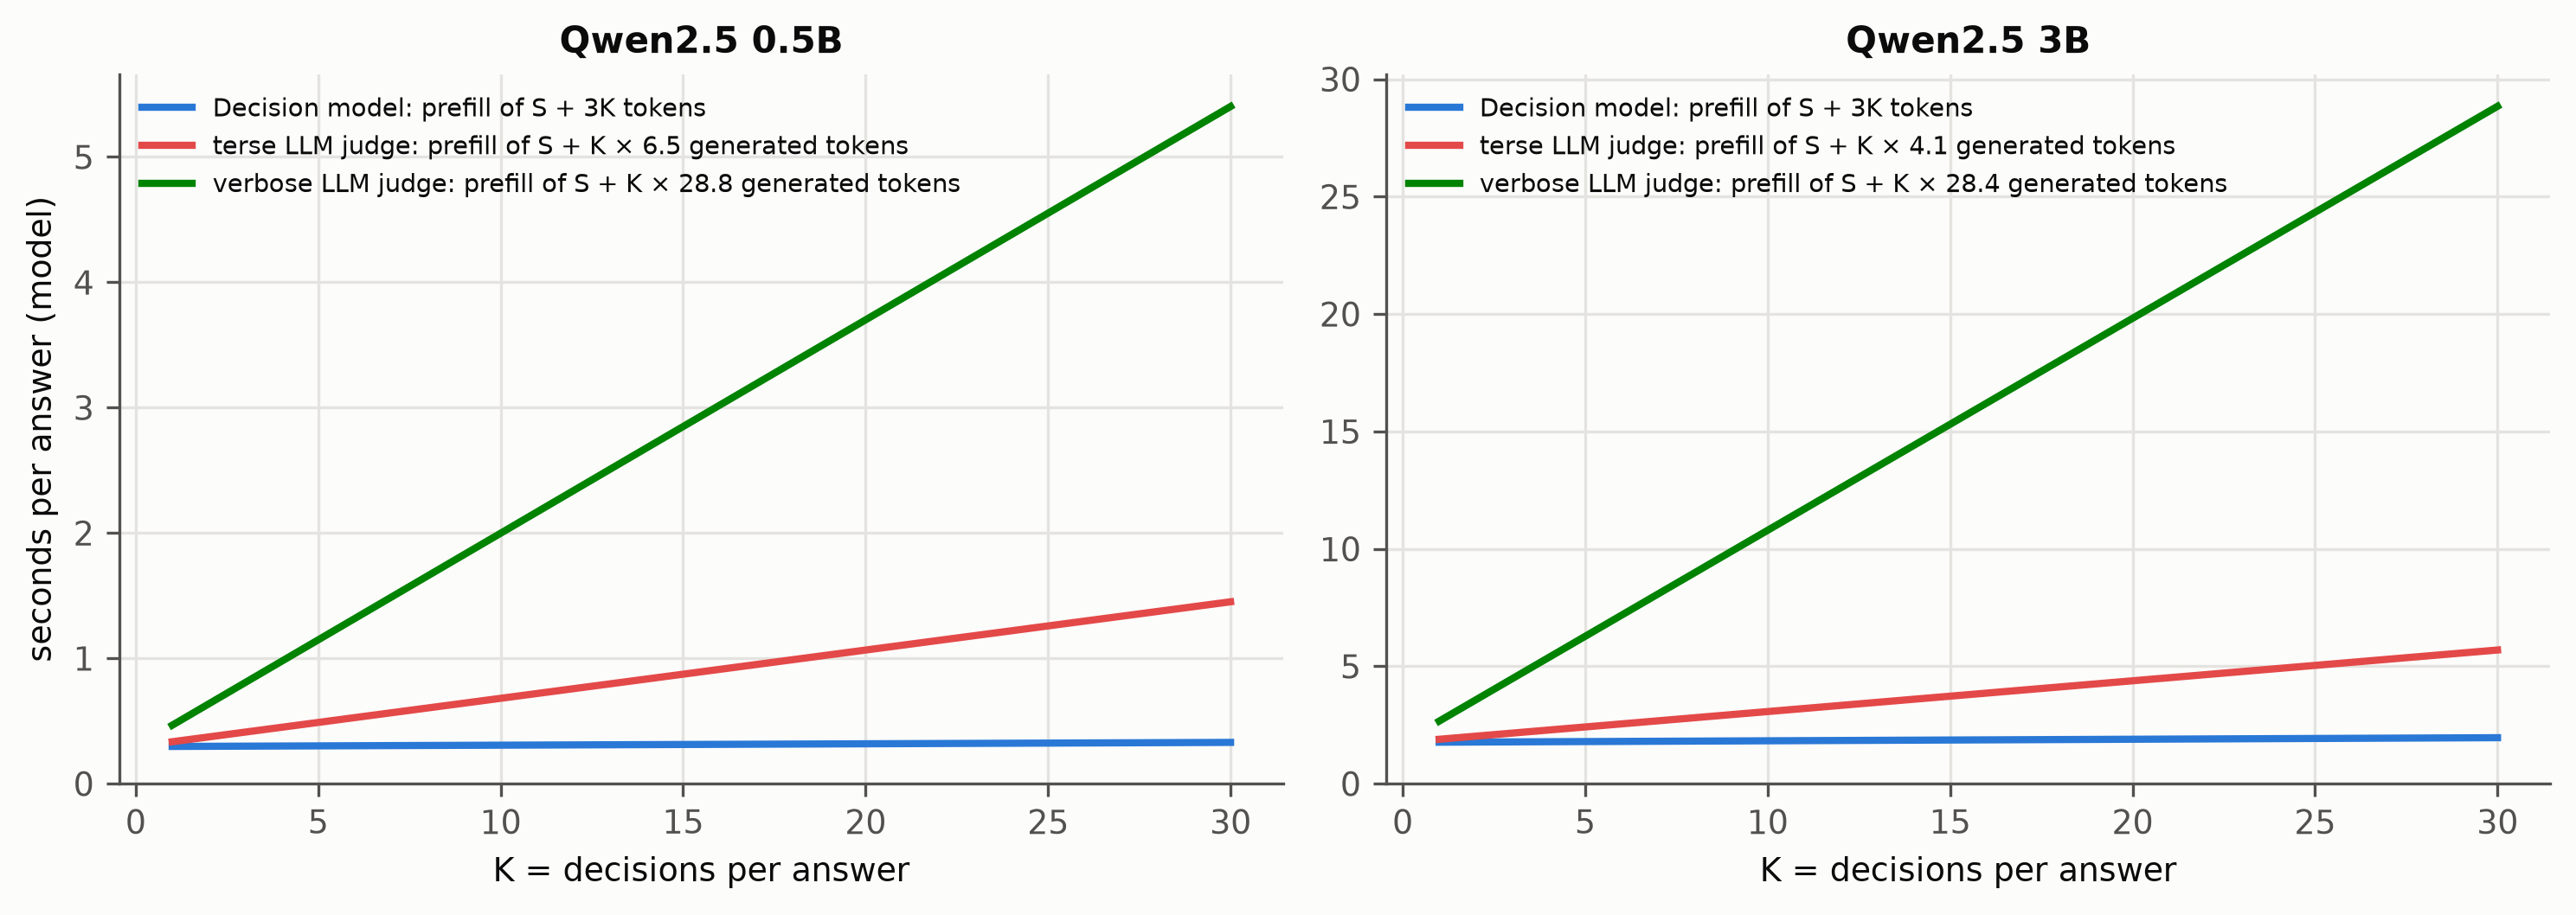
\includegraphics[width=\textwidth]{images/method/cost_model.png}
\caption{Costo stimato della verifica di una risposta di $S = 800$ token in funzione di $K$, calcolato con le sole costanti misurate sull'M4: il tempo per token del prefill e del decoding e il numero medio di token che ciascun giudice genera per verdetto sul sottoinsieme di latenza ($K$ medio 8.7). È un modello analitico, non una misura: le latenze misurate sono nella Sezione~\ref{sec:results-latency}. Il costo del System One cresce di soli tre token di prefill per decisione, quello dei giudici di alcuni token di decoding per decisione.}
\label{fig:method-cost}
\end{figure}

Esiste anche una seconda soluzione, che legge una sola volta il prefisso condiviso e vi accoda poi una breve domanda per
ogni frase, valutando le domande in batch. A differenza della soluzione a marker, che si accontenta di un solo
passaggio, questa richiede però una KV cache replicata $K$ volte. È mantenuta come alternativa di riserva ed è il formato
naturale per un modello non addestrato, che comprende una domanda esplicita ma non ha motivo di interpretare un marker
come una richiesta di verdetto. Per questo è il formato usato dalla baseline non addestrata
(Sezione~\ref{sec:setup-baselines}). La Figura~\ref{fig:method-designs} confronta le due soluzioni.

\begin{figure}[htbp]
\centering
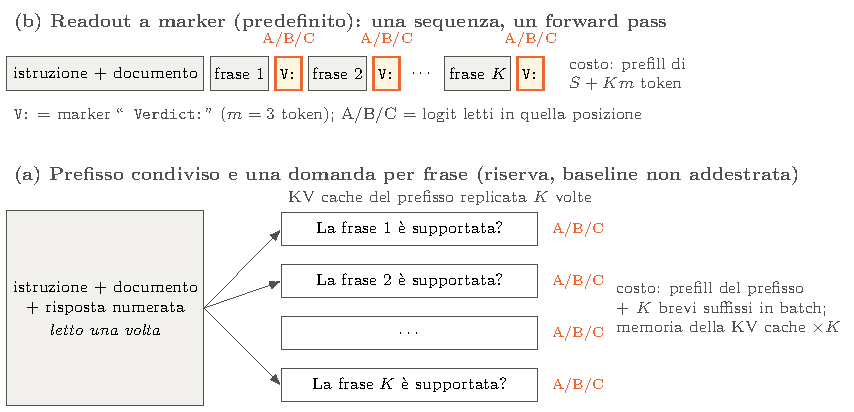
\includegraphics[width=\textwidth]{images/diagrams/method_designs_ab_tikz.pdf}
\caption{Le due soluzioni per ottenere $K$ verdetti da una sola lettura. (b) Il readout a marker, adottato come predefinito, inserisce un marker dopo ogni frase e legge tutti i verdetti nello stesso passaggio. (a) La soluzione di riserva legge una volta il prefisso condiviso e vi accoda una breve domanda per ogni frase, valutate in batch; richiede però $K$ copie della KV cache del prefisso, ed è il formato naturale per un modello non addestrato.}
\label{fig:method-designs}
\end{figure}

\paragraph{Un classificatore, non un generatore più veloce.} Il readout restringe la decisione a tre lettere, e la
restrizione non è un dettaglio. Dopo il marker, il modello sottoposto a fine-tuning non scriverebbe la lettera che viene
letta. Il suo token successivo più probabile è infatti la stessa lettera preceduta da uno spazio, che per il tokenizer è
un token diverso. In corrispondenza dei marker, le tre lettere del readout raccolgono insieme appena il 4--5\,\% circa
della massa di probabilità. Una loss ristretta a queste lettere addestra i loro logit relativi, non la loro probabilità
assoluta, e il readout si comporta quindi come un classificatore a tre classi innestato sul modello linguistico. È
questo a definire un System One: la risposta non passa mai per il decoding, ma viene scelta fra le opzioni ammissibili.
Il fenomeno richiama anche due risultati della letteratura: la probabilità del primo token di risposta e la risposta
effettivamente scritta dal modello possono non coincidere~\cite{wang2024myanswerc}, e la scelta fra lettere è soggetta a
bias di selezione~\cite{zheng2024mcq}. Un readout specializzato e calibrato deve assorbire entrambi gli effetti. Un
esperimento di controllo ne quantifica la differenza rispetto alla generazione: mantiene gli stessi pesi e lo stesso
passaggio, ma al posto del readout ristretto prende il token che la generazione emetterebbe
(Sezione~\ref{sec:results-readout}).

% Marker " Verdict:" = 3 tokens with the Qwen2.5 tokenizer (" Ver", "dict", ":"), verified 2026-10-07.
% Prefill / decode speeds: Phase 0 measurements (Project/docs/phase0_report.md). Readout mass: thesis_notes.md (B2 check).

\section{Obiettivo di addestramento}
\label{sec:method-training}

GroundOne si ottiene da Qwen2.5-0.5B-Instruct e Qwen2.5-3B-Instruct~\cite{qwen2024qwen25} tramite low-rank adaptation
(LoRA)~\cite{hu2022lora}. Gli adapter hanno rango 16, fattore di scala 2 e dropout 0.05\footnote{Il \emph{fattore di
scala} moltiplica l'aggiornamento calcolato dall'adapter prima di sommarlo all'output dello strato congelato. Il
\emph{dropout} azzera a caso, durante l'addestramento, una frazione degli input dell'adapter (qui il 5\,\%), così da
ridurre il rischio che il modello memorizzi il training set.}. Sono applicati a tutti i layer lineari di tutti i blocchi
transformer, perché coprire ogni layer conta più che usare un rango elevato~\cite{dettmers2023qlora}. I pesi del modello
base restano congelati in precisione a 8 bit. Ogni esempio di addestramento è una risposta con tutte le sue frasi
valutate, e la loss viene calcolata su ciascuno dei suoi marker.

La loss è una cross-entropy\footnote{La \emph{cross-entropy} di una predizione è il logaritmo negativo della
probabilità che il modello assegna alla classe corretta: vale zero quando questa probabilità è uno e cresce senza limite
quando il modello sbaglia con sicurezza.} calcolata sulle sole tre lettere. Il prompt non viene mai supervisionato,
quindi il segnale di addestramento proviene interamente dai verdetti. Circa l'88\,\% delle frasi del training set è
supportato, per cui le classi sono pesate in modo che ciascuna contribuisca in egual misura alla loss. Con la
distribuzione del training set si ottengono pesi di circa 0.38 per le frasi supportate, 7.5 per quelle contraddette e 4.4
per quelle non menzionate. Senza questi pesi, un modello può ottenere una loss bassa rispondendo quasi sempre
``supportata''. Ne discende una conseguenza utile: un modello che avesse appreso soltanto le frequenze delle classi
resterebbe a una loss di $\ln 3 \approx 1.10$, quindi una loss inferiore a questo valore indica che il modello sfrutta
effettivamente il testo.

L'ottimizzatore è AdamW, usato senza weight decay, cioè senza la penalità che a ogni passo riduce l'ampiezza dei pesi.
Come nella configurazione predefinita di MLX, le stime dei momenti non ricevono la bias correction, e non si applica
gradient clipping. L'addestramento dura un'epoca, cioè un solo passaggio sulle risposte del training set. Il learning
rate sale fino a $10^{-4}$ con un warm-up lineare sul primo 3\,\% dei passi e poi scende fino a zero con un cosine
schedule\footnote{Durante il \emph{warm-up} il learning rate cresce gradualmente fino al valore scelto, così da evitare
aggiornamenti bruschi all'inizio dell'addestramento. Il \emph{cosine schedule} lo riduce poi seguendo mezzo periodo di
un coseno: lentamente all'inizio, più in fretta a metà e di nuovo lentamente verso la fine.}. Le risposte di lunghezza
simile sono raggruppate in micro-batch, ciascuno entro un budget di token che comprende anche il padding, cioè i token di
riempimento che uniformano le lunghezze. I gradienti di più micro-batch vengono poi accumulati, in modo che ogni passo
dell'ottimizzatore veda circa 16 risposte, ovvero circa 110 decisioni. Così ogni passo contiene qualche frase
contraddetta, nonostante la rarità della classe. Il gradient checkpointing, che durante il calcolo dei gradienti
ricalcola alcune attivazioni invece di conservarle, mantiene l'occupazione di memoria entro i 16\,GB del portatile.
Durante l'addestramento il modello viene valutato periodicamente sul dev set, e si conserva il checkpoint, cioè la copia
dei pesi, con la balanced accuracy a tre classi più alta, mediata sui tre task di RAGTruth (question answering, summarization e data-to-text). La Sezione~\ref{sec:setup-models} riporta
le impostazioni di ciascun run.

\section{Calibrazione}
\label{sec:method-calibration}

I pesi delle classi addestrano il modello come se le tre classi fossero ugualmente frequenti, per cui le sue
probabilità grezze non rispecchiano le frequenze reali delle classi. Sul dev set si stima quindi una trasformazione
post-hoc, applicata ai logit dopo l'addestramento e senza modificare i pesi. I tre logit vengono divisi per una
temperatura $T$ e traslati di un bias per classe, $\mathrm{softmax}(z / T + b)$, con il bias della classe supportata
fissato a zero. I parametri $T$ e $b$ sono scelti minimizzando la negative log-likelihood delle etichette del dev set,
cioè la cross-entropy media~\cite{guo2017calibration}. Il bias svolge il ruolo della correzione contestuale proposta per
i modelli linguistici interrogati tramite prompt~\cite{zhao2021calibrate}; a differenza di quella, però, qui è stimato
su dati etichettati. La sola temperatura cambia le probabilità ma non la classe più probabile né l'ordinamento delle
frasi. Il bias, invece, può cambiare la classe più probabile e, con tre classi, può anche riordinare leggermente
$P(\text{supported})$ fra una frase e l'altra. Per questo le metriche di classificazione e
l'AUROC\footnote{L'\emph{AUROC} è l'area sotto la curva ROC e misura quanto bene un punteggio ordina gli esempi:
equivale alla probabilità che un esempio positivo scelto a caso riceva un punteggio più alto di un esempio negativo
scelto a caso. Vale 0.5 per un punteggio casuale e 1 per un ordinamento perfetto, e non dipende da alcuna soglia.} sono
calcolate sull'output grezzo. Le probabilità calibrate si usano invece dove una probabilità deve corrispondere a una
frequenza: nelle metriche di calibrazione, nelle soglie e nella selective prediction
(Sezione~\ref{sec:results-calibration}).

La calibrazione è misurata principalmente con l'Expected Calibration Error
(ECE)~\cite{naeini2015ece,guo2017calibration}. Le predizioni vengono ripartite in base alla confidenza in $M$
intervalli di uguale ampiezza, con $M = 15$ in questa tesi. Per ogni intervallo $B_m$ si confronta la confidenza media
$\mathrm{conf}(B_m)$ con la frequenza osservata $\mathrm{acc}(B_m)$, e gli scarti vengono mediati con pesi
proporzionali alla numerosità degli intervalli:
\begin{equation}
  \mathrm{ECE} = \sum_{m=1}^{M} \frac{|B_m|}{n} \, \bigl| \mathrm{acc}(B_m) - \mathrm{conf}(B_m) \bigr| .
\end{equation}
Qui $n$ è il numero complessivo di predizioni. Nella variante binaria la confidenza è $P(\text{supported})$ e la
frequenza osservata è la quota di frasi supportate nell'intervallo. Nella variante top-label a tre classi, invece, la
confidenza è la probabilità massima e la frequenza osservata è la quota di predizioni corrette. L'ECE non confronta la
distribuzione delle classi predette con quella del test set. Verifica piuttosto se, fra le frasi a cui il modello
assegna una certa confidenza, quella confidenza corrisponde alla realtà. La misura ha però due limiti: dipende dalla
scelta degli intervalli, e un predittore costante che restituisce sempre la frequenza di base ottiene un ECE vicino a
zero pur non discriminando nulla. Per questi motivi l'ECE è sempre riportato insieme al Brier score\footnote{Il
\emph{Brier score} è l'errore quadratico medio fra la probabilità predetta e l'esito osservato, codificato come 1 se
l'evento si verifica e 0 altrimenti: più è basso, migliori sono le probabilità.}, alla negative log-likelihood e ai
reliability diagram, i grafici che riportano per ogni intervallo la frequenza osservata in funzione della confidenza
media. La capacità delle probabilità di separare le decisioni corrette da quelle errate si misura invece a parte, con
l'AUROC e con l'area sotto la risk--coverage curve.

\paragraph{Dalle probabilità alle etichette restituite.} Chi usa il verificatore vede per ogni frase un'etichetta e una
probabilità, che devono essere coerenti tra loro. Questa tesi valuta la decisione grezza, cioè la classe più probabile
secondo l'output non calibrato. La decisione grezza, però, può contraddire la probabilità calibrata mostrata accanto: una
frase può essere etichettata ``non menzionata'' pur avendo una $P(\text{supported})$ calibrata di poco superiore a un
mezzo. L'output restituito ricava quindi ogni elemento dalle probabilità calibrate con un'unica regola. Una frase è
etichettata come supportata se e solo se $P(\text{supported}) \geq \tau$; altrimenti riceve la più probabile fra le due
classi restanti. La policy strict segnala ogni frase non supportata, quella lenient soltanto le contraddette. La soglia
$\tau$ è stimata sul dev set in modo da massimizzare la balanced accuracy a tre classi. L'utente può modificarla a ogni
richiesta, scegliendo così un diverso punto operativo senza riaddestrare il modello. La Figura~\ref{fig:method-calflow} riassume il percorso dai logit grezzi alle etichette restituite.

\begin{figure}[htbp]
\centering
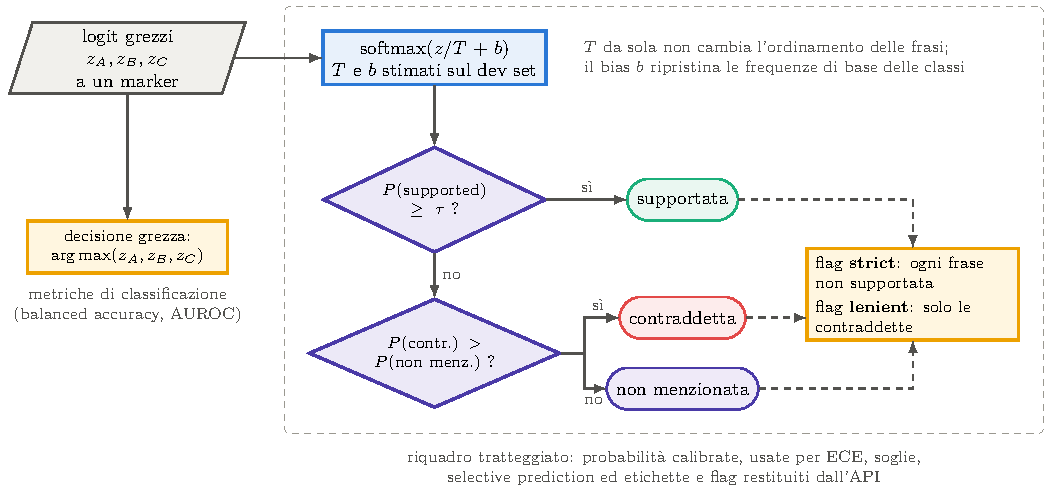
\includegraphics[width=\textwidth]{images/diagrams/method_calibration_flow_tikz.pdf}
\caption{Dai logit alle etichette restituite. La decisione grezza, cioè l'argmax dei logit, serve alle metriche di classificazione del Capitolo~\ref{sec:results}. Le probabilità calibrate, ottenute con temperatura e bias stimati sul dev set, alimentano invece l'unica regola dell'output restituito: supportata se $P(\text{supported}) \geq \tau$, altrimenti la più probabile fra contraddetta e non menzionata. Da qui derivano i flag strict e lenient.}
\label{fig:method-calflow}
\end{figure}

\section{Software}
\label{sec:method-software}

GroundOne è implementato come pacchetto Python installabile basato su MLX~\cite{mlx2023,mlxlm}, il framework per array
pensato per Apple silicon. Tutte le fasi di addestramento e di inferenza descritte finora vengono eseguite con MLX sullo
stesso portatile. Il pacchetto comprende il costruttore del dataset con i relativi controlli, il ciclo di addestramento,
la calibrazione, la valutazione sui test set congelati, le baseline e un meccanismo di protezione della memoria.
Quest'ultimo esegue i processi lunghi uno alla volta e interrompe un processo prima che il sistema esaurisca la memoria.

Il verificatore è esposto tramite un'interfaccia a riga di comando e un server HTTP. Il server offre un endpoint nativo e
un endpoint compatibile con l'interfaccia usata da altri modelli System One, così che i client esistenti possano adottare
GroundOne cambiando soltanto l'indirizzo. L'endpoint nativo riceve un documento e una risposta. Segmenta la risposta con
la stessa regola usata per costruire i dati ed esegue il singolo forward pass della Sezione~\ref{sec:method-readout}. Per
ogni frase riporta se è stata valutata, le tre probabilità calibrate, l'etichetta restituita e i flag delle policy
strict e lenient, insieme alla regola di decisione e alla soglia che li hanno prodotti. Indica inoltre il numero di token
in ingresso, il numero di token generati, sempre pari a zero, e il tempo impiegato. L'endpoint compatibile, invece,
risponde a domande chiuse generiche su un contesto condiviso, con il formato a una domanda per frase. Tutto il calcolo del
modello avviene su un unico worker thread di lunga durata, perché il contesto Metal della GPU, cioè lo stato con cui il
programma la usa attraverso l'interfaccia grafica di Apple, non deve spostarsi da un thread all'altro. Infine, nulla esce
dalla macchina: modelli, dati e richieste restano in locale. La Figura~\ref{fig:method-software} riassume l'architettura del pacchetto.

\begin{figure}[htbp]
\centering
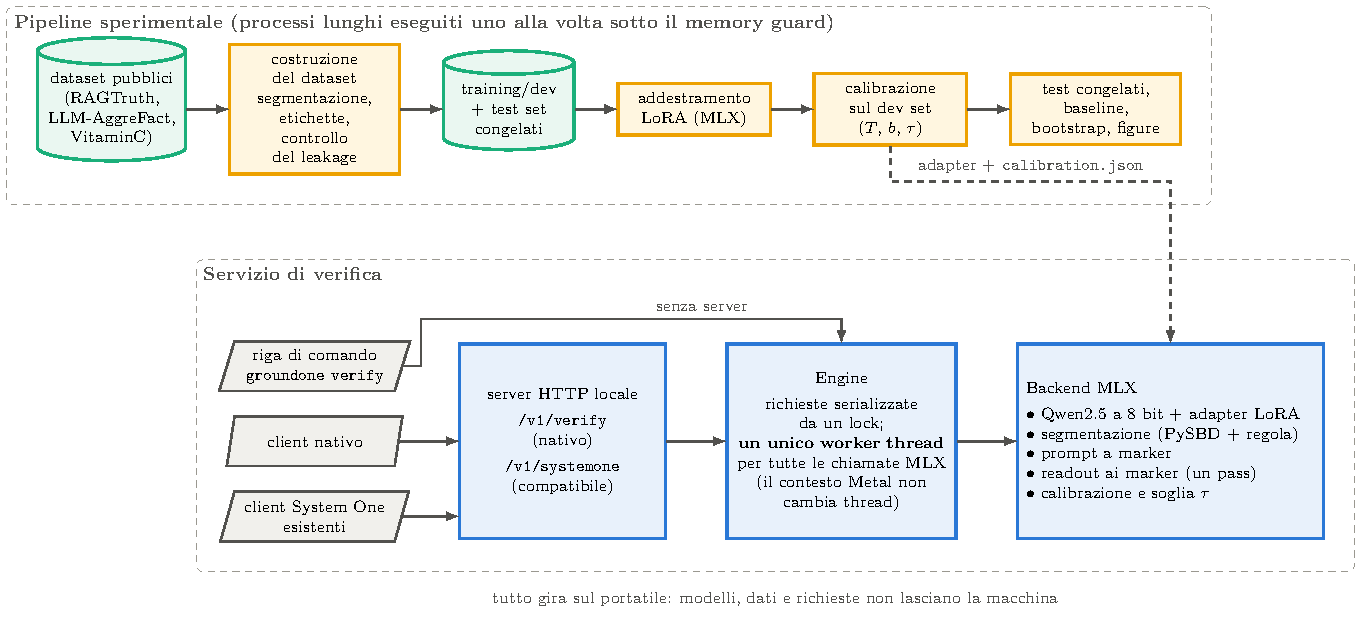
\includegraphics[width=\textwidth]{images/diagrams/method_software_tikz.pdf}
\caption{Architettura del software. In alto la pipeline sperimentale, dai dataset pubblici ai test congelati, eseguita sotto il memory guard; in basso il servizio di verifica, in cui riga di comando e server HTTP (endpoint nativo e compatibile) condividono lo stesso Engine, che serializza le richieste ed esegue ogni chiamata MLX su un unico worker thread. L'adapter e il file di calibrazione prodotti dalla pipeline sono gli unici artefatti che il servizio legge.}
\label{fig:method-software}
\end{figure}
